\section{Current EIDA processing and validation}

The current eligible continuous-observation checkpoint contains 246,668 picks and 3,271 provisional associations from 1,285 files and 13,467.933 channel-hours. 2996 associations have causal usable arrivals; 552 meet the numerical calibration selection. 1435 locations pass VELEST filters and 1050 remain after both TomoDD rounds and the gap filter. All known event-selected snippets are excluded. These calculations remain provisional; filter passage does not establish correct event identity or fault geometry.

Relative to the preserved previous checkpoint, retained trial events increased from 123 to 1050. Conditional SVD estimates increased from 80 to 352; median vertical uncertainty changed from 233.4 to 244.6 m and the maximum from 1336.6 to 3499.1 m. The cohorts differ, so these changes do not establish improved location accuracy. Current depth quantiles and year counts are saved in result\_summary.json; no accepted caldera geometry or depth limit is inferred.

New requests: {'downloaded': 275, 'no\_data': 1}; 3.481 GB returned. 73,641 requests remain unattempted; this is unfinished acquisition, not a remote-access failure. The batch prioritizes final study days, then calendar-selected dates across years. An additional 20-station batch covers the full 2024-05-20 18:00 to 2024-05-21 00:00 UTC interval containing the S4 benchmark. This purposeful continuous-window sampling does not establish discovery of the known swarm or population completeness. Original files, checksums and request outcomes are saved. RAN access and the exact Calo--Tramelli profile were deferred as instructed.

\par\path{data/eida_continuation/request_ledger.csv.gz}\par\path{data/eida_continuation/station_coverage.csv}\par\path{data/eida_continuation/unobserved_channel_intervals.csv}

Response epochs cover 13467.933 observed channel-hours; 0.000000 hours lack complete responses. The 14 event-selected files remain preserved for labeled waveform checks; they do not supply independent continuous detections or completeness statistics.

The 165 original baseline files retain their earlier 15-second inference margins; new segmented inference uses 30 seconds. Original waveform, configuration and saved-pick hashes were verified. Known event-selected windows are excluded from both detections and exposure. Reduced station count relative to the previous checkpoint reflects that exclusion, not loss of downloaded continuous records.

\subsection*{Location validation}

The unconstrained new-cohort fits had negative isotropic bulk modulus in the 3--5 km layer (Vp/Vs 1.073 and 1.088). Those outputs and the interrupted relocation attempt are preserved in unconstrained\_calibration.zip. The current fit uses one disclosed increase to uniform velocity-layer damping 100, motivated by that failure and generic VELEST regularization guidance. No observations or acceptance limits changed. The resulting velocities are strongly influenced by the starting grid; physical admissibility does not establish data resolution or exact reproduction.

Calibration dates: {'2022-01-21': 1, '2022-01-24': 2, '2022-01-25': 1, '2022-01-26': 2, '2022-01-28': 1, '2022-02-01': 2, '2022-03-01': 1, '2023-03-01': 6, '2024-02-01': 9, '2024-04-01': 1, '2024-05-20': 464, '2025-01-01': 1, '2025-02-01': 6, '2025-03-18': 24, '2025-03-19': 14, '2025-03-20': 17}. The chronological every-fifth-event holdout is interleaved within the sampled swarms; it is not an independent out-of-region or out-of-period accuracy test.

Separating fixed-model events into batches was rejected after a 1.91 km maximum depth change. Production retains global VELEST updates. A zero-term Cholesky optimization reproduced six complete 552-event, 9,529-phase runs byte for byte, including location, velocity, station-correction and residual files. A further 32-bit dense comparison of current fixed-model prelocation is also byte-identical. Both arithmetic precisions use this checked optimization. Numerical equivalence is distinct from accuracy.

TomoDD storage was expanded to accommodate the measured phase pairs. Zero-correlation diagnostic logging errors in generic TomoDD and HypoDD were corrected without changing inverse equations. The first TomoDD cluster remained byte-identical through all eight iterations; a successful HypoDD component also remained byte-identical. The repaired small SVD component returned three additional estimates; the component rejected as airquakes was not forced to return a solution.

\par\path{data/eida_continuation/tomodd_logging_fix_check.json}\par\path{data/eida_continuation/hypodd_logging_repair.json}

\par\path{data/eida_continuation/sparse_check.json}\par\path{data/eida_continuation/unconstrained_archive.json}\par\path{config/eida_calibration.json}

Full precision paths differ by 1075.2 m horizontally and 0.850 km in depth; precision gate: False. Regional-start depth difference: 1.520 km. Held-out refitting uses 441 training and 111 withheld events. Held-out RMS changes from 0.2403 to 0.2081 s.

TomoDD inter-round maximum change is 1830.3 m horizontally and 1.154 km vertically. 404 retained events have no waveform-correlation links. SVD errors are conditional on the fitted model and phase assignments, and exclude these systematic uncertainties. Generic HypoDD also clips the negative CFB1/CFB3 elevations to sea level, omitting 40.4/38.7 m of receiver depth; the original metadata and this approximation are recorded in receiver\_convention\_check.json. The corrected S9 threshold is $>$=100, following the supplement's exclusion of sums below 100; no gate was weakened to create a result.

Compared with the previous 123-event trial, the current trial has 1050 events. Reciprocal origin-time matching ($<$2 s, no author catalog) links 22 events. This is a change diagnostic, not an accuracy measurement. Independent S--P checks use 4368 measurements with RMS discrepancy 0.1820 s against the own approximate model.

The precision runs use identical observations, initial files and controls. A 150 m maximum depth difference already occurs during fixed-model prelocation. The final median difference is 40 m and the 95th percentile is 273 m, with a maximum of 850 m. Common intermediate starts reduce some differences but do not remove them. The exact ill-conditioned mode or ray switch was not isolated, and these differences are not treated as harmless rounding.

\par\path{data/eida_continuation/precision_diagnosis.csv}

\par\path{data/eida_continuation/calibration/merged4/heldout/summary.json}\par\path{data/eida_continuation/calibration/merged4/validation.json}\par\path{data/eida_continuation/calibration/merged4/uncertainty/summary.json}

\subsection*{Template and frequency-index screening}

1843 unconfirmed template-score crossings over 140.656 common CAAM/COLB hours. Twelve highest scores per template displayed from original waveforms with measured frequency indices and amplitude ratios. No confirmed cluster or accepted hybrid magnitude. AI inspection of 36 displayed crossings found 4 preceding-packet tails and 3 ongoing-activity windows; the other transients remain unclassified. No human review.

\par\path{data/eida_continuation/hybrid/provenance.json}\par\path{data/eida_continuation/hybrid/visual_review.csv}

The written-method template times select original waveform examples only. These templates never enter the continuous detection catalog or exposure. Other score crossings remain unreviewed; no verified three-year hybrid chronology or family magnitudes are available.

Phase support in the retained relocated set: {'events': 1050, 'no\_P': 5, 'fewer\_than\_four\_P': 396, 'no\_S': 0, 'P': 5225, 'S': 8079}. S-only or P-poor associations have weak independent control on origin time and absolute depth. The published six-pick gate is retained; these diagnostics are disclosed rather than silently adding a new selection.

\subsection*{Mechanisms}

Before visual review, automatic first-motion screening evaluated 197 events and 1969 station windows; 12 events had at least eight stable automatic signs. The unchanged SKHASH geometry gates returned 0 mechanisms. These automatic signs are not counted as visually reviewed measurements.

12 unaccepted own FK/gCAP trial fits using newly available EIDA records and the current own model and explicitly linked own candidate geometry. 99 AI-reviewed polarities, 108 AI-reviewed ratios; no human review. SKHASH returns 2 solutions. Low-band variance reduction 1.3--14.4\%; orientations change 45.0--95.0 degrees between frequency bands. Gray beachballs denote unvalidated trials; background is the new independent catalog, never joined to candidates by integer ID. SKHASH returns 2 quality-D trials. No scientifically accepted mechanism.

\begin{center}\small\begin{tabular}{rrrrl}\toprule Candidate & P & S/P & Azimuth gap & Requirement\\\midrule

212 & 3 & 5 & 175.5 & Fewer than 8 P\\

312 & 5 & 5 & 155.9 & Fewer than 8 P\\

315 & 4 & 4 & 252.9 & Fewer than 8 P\\

359 & 4 & 8 & 165.4 & Fewer than 8 P\\

373 & 3 & 5 & 177.8 & Fewer than 8 P\\

649 & 8 & 10 & 120.5 & Geometry/model validation\\

698 & 1 & 1 & 360.0 & Fewer than 8 P\\

815 & 4 & 6 & 167.1 & Fewer than 8 P\\

100331 & 16 & 12 & 103.6 & Geometry/model validation\\

100946 & 17 & 13 & 95.3 & Geometry/model validation\\

100948 & 0 & 0 & 360.0 & Fewer than 8 P\\

101038 & 11 & 15 & 90.3 & Geometry/model validation\\

101400 & 14 & 16 & 83.6 & Geometry/model validation\\

101760 & 9 & 8 & 84.0 & Geometry/model validation\\

\bottomrule\end{tabular}\end{center}

\par\path{data/mechanism_eida/review_transfer.json}\par\path{data/mechanism_eida/review_decisions.csv}\par\path{data/mechanism_eida/skhash.log}\par\path{data/mechanism_eida/gcap_band_sensitivity.csv}

Prior review decisions are retained only after explicit observation-window equality checks; new or changed windows receive a separate AI review record. Zero human reviews are claimed. Candidate labels preserve earlier review IDs; the shared-phase mapping identifies current locations and explicitly marks any retained historical location. The new model and all locations remain provisional. Event-dependent filters and source controls are exploratory; neither weak fits nor a returned solver file establishes a reliable mechanism.

\begin{center}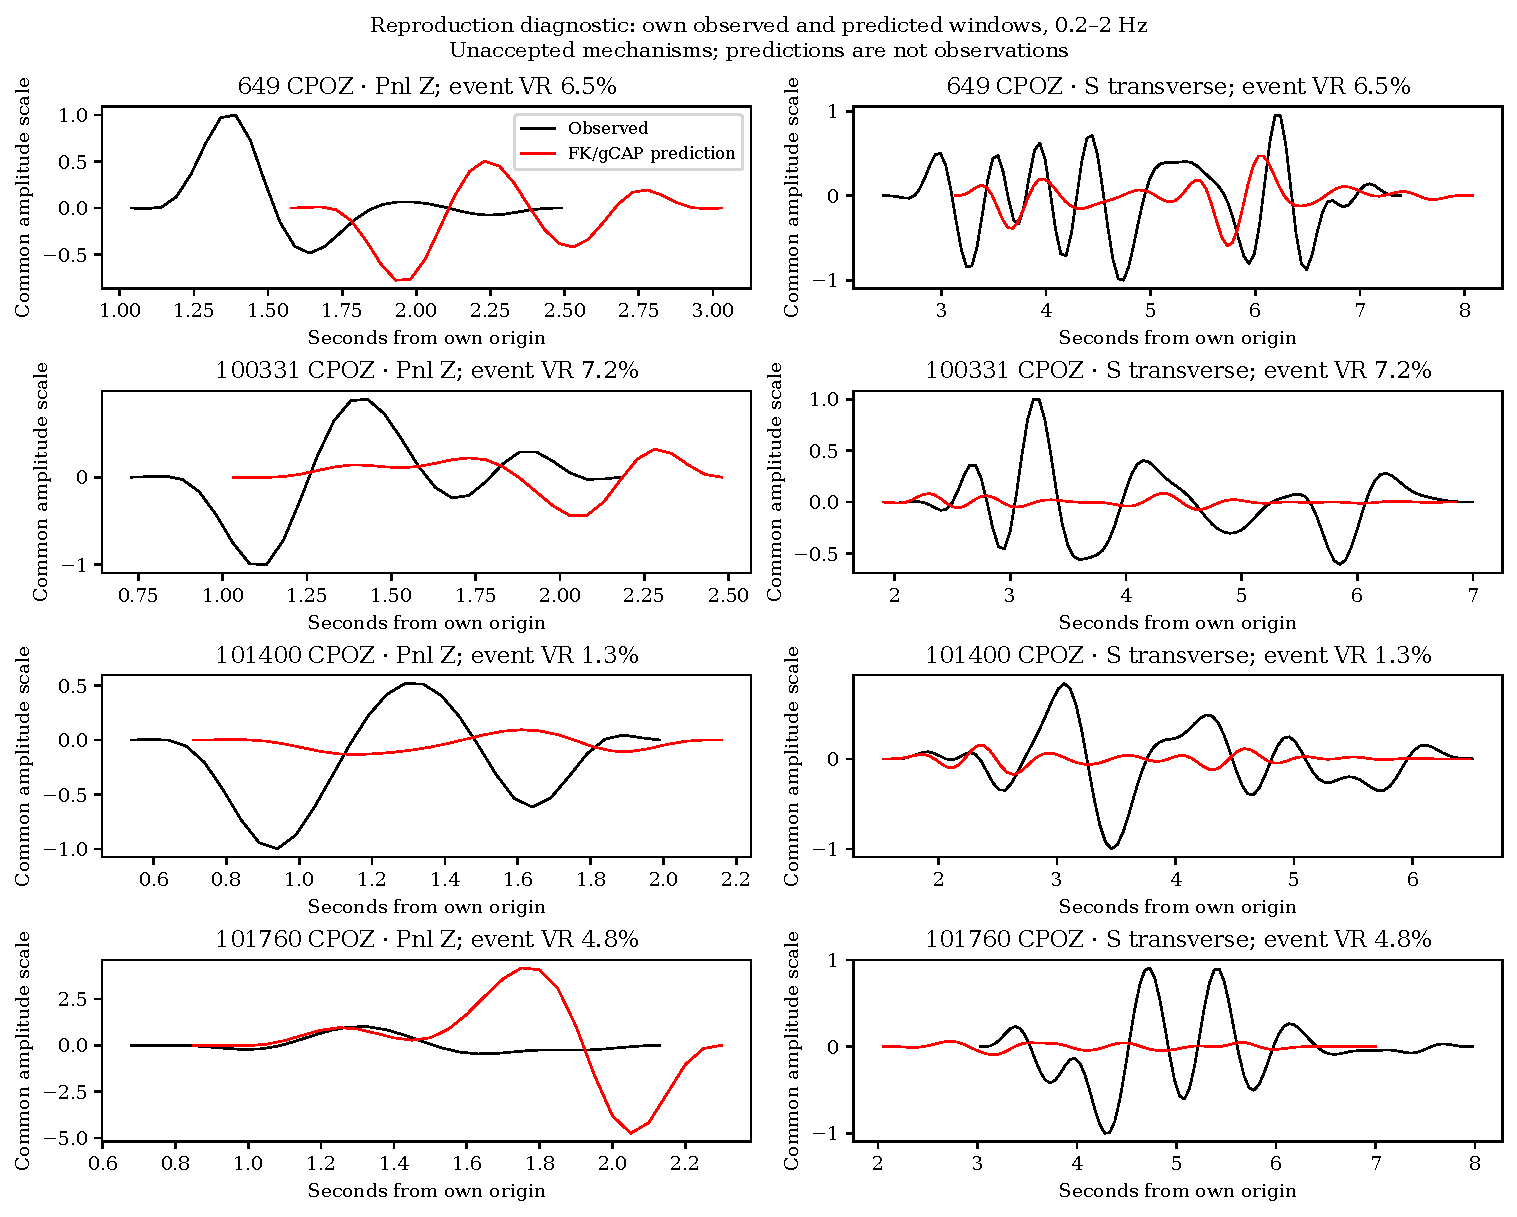
\includegraphics[width=.95\linewidth]{figures/mechanism_eida_fit_diagnostic.pdf}\end{center}

Reproduction diagnostic, not a publication figure. CPOZ observations and own FK/gCAP predictions for four explicitly selected trial events share one amplitude normalization per pair. Red curves are theoretical predictions, not observational or synthetic fixture data. Predicted amplitudes are not normalized separately. Saved fitted lags are included; weak event variance reduction and band dependence prevent mechanism acceptance.

Own SKHASH--gCAP Kagan angles span 35.6--79.1 degrees across 4 event/band pairs. These trial comparisons do not establish the paper's high-quality selection because locations, phase identity and model sensitivity remain unresolved.

\par\path{data/mechanism_eida/skhash_gcap_comparison.csv}\par\path{data/mechanism_eida/candidate_requirements.csv}

Eight additional downstream-only P arrival marks were inspected against raw and response-corrected traces; seven first-motion signs were retained. CPOZ supplies three additional clear P/S packets. These AI arrivals do not enter the detection or association catalog. Candidate 100948 has unresolved identity amid preceding activity, about 14 seconds after a larger candidate; all its amplitude measurements fail quality control. Near/pre-origin CAAM/COLB motion for candidate 101760 flags an association/origin inconsistency. Neither candidate is silently removed or accepted as a validated event.

\par\path{config/mechanism_eida_arrivals.csv}\par\path{data/mechanism_eida/new_visual_review.json}\par\path{data/eida_continuation/catalog_quality_flags.csv}

\subsection*{Rebuild and preserved checkpoints}

Run \texttt{.venv/bin/python\allowbreak{} scripts/rebuild\_eida\_followup.py\allowbreak{} --analysis} for the frozen observation set, or omit \path{--analysis} to verify saved numerical files and rebuild figures and both PDFs. Retrieval is separate: \texttt{.venv/bin/python\allowbreak{} scripts/collect\_eida\_followup.py\allowbreak{} --max-jobs\allowbreak{} 256\allowbreak{} --workers\allowbreak{} 4}. It selects only pending, never-attempted requests. The command does not retry prior empty or failed intervals. Actual execution and build outcomes are in \path{data/eida_continuation/pipeline_execution.json} and \path{data/eida_continuation/rebuild_result.json}.

Earlier data/local\_extension, data/coverage\_extension and data/mechanism\_followup remain preserved, with their distinct identifiers and superseded figures. The main report, comparison PDF, panel records and current figure fragments are updated; no published-result tables enter the calculation. Existing historical/context, training-example and original-region-mask limitations are unchanged.

\subsection*{Current panel summary}

Partial: 1A, 1B, 1C, 2A, 2B, 3/map, 3/northing-depth, 3/easting-depth, 4A, 4B, S1, S2, S4A, S5/map, S5/northing-depth, S5/easting-depth, S6/map, S6/northing-depth, S6/easting-depth, S7A/map, S7A/easting-depth, S7B, S7D, S7F, S7C, S7E, S7G, S8A, S8B, S10/2022, S10/2023, S10/2024, S10/2025, S11/swarm-1, S11/swarm-2, S11/swarm-3, S12A, S12B, S12C, S12D, S12E, S12F, S12G, S12H, S13A, S13B, S14/1, S14/2, S14/3, S15A, S15B, S15C, S15D. Unreproduced: S3A, S3B, S3C, S3D, S4B, S9/map, S9/northing-depth, S9/easting-depth, S11/swarm-4, S14/unclustered. No full independent reproduction is claimed.
